\documentclass[letterpaper,10pt,onecolumn]{article}
\usepackage[spanish]{babel}
\usepackage[utf8x]{inputenc}
\usepackage{amsfonts}
\usepackage{amsthm}
\usepackage{amsmath}
\usepackage{mathrsfs}
\usepackage{empheq}
\usepackage{enumitem}
\usepackage[pdftex]{color,graphicx}
\usepackage{hyperref}
\usepackage{listings}
\usepackage{calligra}
\usepackage{algpseudocode} 
\DeclareMathAlphabet{\mathcalligra}{T1}{calligra}{m}{n}
\DeclareFontShape{T1}{calligra}{m}{n}{<->s*[2.2]callig15}{}
\newcommand{\scripty}[1]{\ensuremath{\mathcalligra{#1}}}
\lstloadlanguages{[5.2]Mathematica}
\setlength{\oddsidemargin}{0cm}
\setlength{\textwidth}{490pt}
\setlength{\topmargin}{-40pt}
\addtolength{\hoffset}{-0.3cm}
\addtolength{\textheight}{4cm}

\begin{document}
\begin{center}



\includegraphics[width=490pt]{header.png}\\[0.5cm]

\textsc{\LARGE Taller 5 - F\'isica I (FISI-1018) - 2016-10}\\[0.5cm]

\textsc{\Large{Profesor: Jaime Forero}} \\[0.5cm]

\noindent\textsc{Ejercicios correspondiente a la clase complementaria de la semana del 22 de Febrero del 2016.}\\[0.5cm]
\end{center}

\noindent\textsc{Nota:} 
Los primeros tres ejercicios deben ser
entregados {\bf al comienzo} de la clase complementaria. Los \'ultimos
cuatro deben ser trabajados {\bf durante} la complementaria. 

La numeraci\'on
hace referencia al texto gu\'ia: \textit{F\'isica Universitaria Volumen
  1 (Sears-Semansky)}, decimotercera edici\'on, Pearson.

\begin{enumerate}
% aqui vienen los tres ejercicios "faciles"
\item Ejercicio 4.23 Dos cajas en contacto.
\item Ejercicio 4.35 Dos caballos
\item Ejercicio 5.2  Tensión de las cuerdas. %Juan Carlos

% aqui vienen los cuatro ejercicios "dificiles"
\item Ejercicio 4.41 Biomec\'anica humana.

\item Un bulto de cemento, cuyo peso es 325 N, cuelga de tres cables como se muestra en la figura. Los angulos que forman las cuerdas con el techo son $\theta_1=60^\circ$ y $\theta_1=40^\circ$, respectivamente. Si se asume que el sistema está en equilibrio, ¿cuáles son las tensiones $T_1$, $T_2$ y $T_3$?

\begin{figure}[hb]
\centering
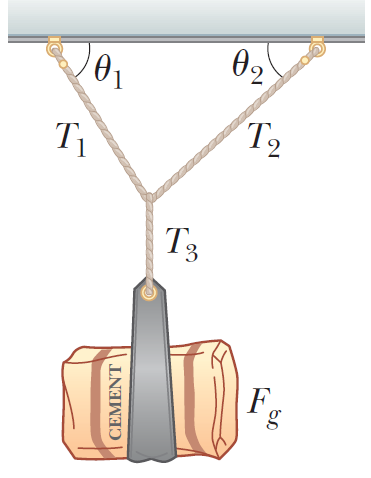
\includegraphics[width=0.35\textwidth]{cemento.PNG}\\
\caption{Diagrama para el problema del bulto de cemento}
\end{figure} %Juan Carlos

\item
La barra que se muestra en la figura 2 (denotada por $AB$), esta sostenida por el cable $BC$, el cual tiene un extremo fijo en el punto $C$. Una persona aplica una fuerza de $50kg$ a lo largo de BD con un ángulo de ($20^{\circ}$) respecto a la vertical. 
\begin{figure}[h]
\centering
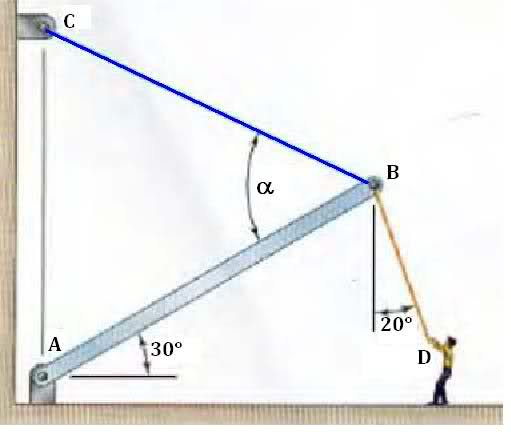
\includegraphics[width=0.35\textwidth]{complementariai1.jpg}\\
\caption{Figura de la barra y el cable}
\end{figure}
\begin{enumerate}
\item 
Determine el valor de $\alpha$ para el cual la tensión es mínima en el cable.
\item
Encuentre la magnitud de la tensión para el ángulo que encontró en el inciso anterior. 
\end{enumerate}
%Miguel

\item
Encontrar el peso necesario en el punto $P$ con el cual se mantendrá en en equilibrio el sistema que se muestra en la figura 3. En este caso $A$ pesa $98kg$ y $Q$ pesa $9.8kg$. La cuerda AC es horizontal y la cuerda $AB$ es paralela al plano.
\begin{figure}[h]
\centering
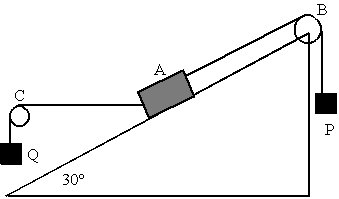
\includegraphics[width=0.35\textwidth]{complementaria02.jpg}\\
\caption{Problema del plano inclinado.}
\end{figure}
\begin{enumerate}
\item 
Realice el respectivo diagrama de fuerzas.
\item
Halle la normal sobre el cuerpo $A$. 
\end{enumerate}
%Miguel 

\end{enumerate}

\end{document}

\begin{figure}[!h]
\begin{center}
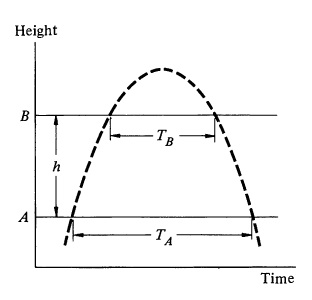
\includegraphics[scale=0.7]{altura.jpg} 
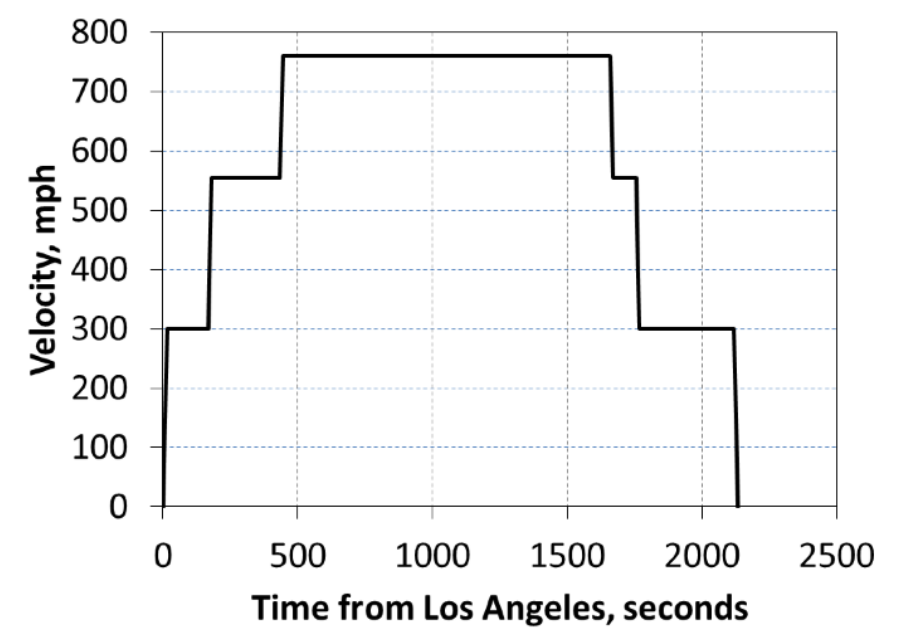
\includegraphics[scale=0.3]{hyperloop.png} 
\end{center}
\caption{Izquierda: diagrama para el ejercicio recomendado 3. Derecha: diagrama para el ejercicio recomendado 4.}
\label{fig:tiro}
\end{figure}





